\chapter{Na\"ieve legoblokdetectie}
\label{hoofdstuk:2}
In dit hoofdstuk bespreken we een na\"ief algoritme om legoblokken te detecteren. Dit algoritme zal op basis van kleurthresholding de legoblokken in de afbeelding lokaliseren en vervolgens op basis van de geometrie van een legoblok de pose bepalen. Hierna vereenvoudigen we dit algoritme door in plaats van expliciet de pose van een legoblok te bepalen gebruik te maken van het grid van de virtuele wereld in ons AR spel. Ten slotte breiden we deze vereenvoudiging uit met een effici\"enter algoritme voor het zoeken van een pad in de virtuele wereld, wat de performantie ten goede komt.

In sectie \ref{sec:naive_begr} worden eerst enkele begrippen uitgelegd. Vervolgens wordt het na\"ieve blokdetectie algoritme uitgelegd in sectie \ref{sec:naive_algo}. Sectie \ref{sec:naive_algo_result} bespreekt dan de implementatie, resultaten en evaluatie van dit algoritme. Verder wordt in sectie \ref{sec:naive_vereenv} de vereenvoudiging van het algoritme behandeld. De uitbreiding op de vereenvoudiging wordt uitgelegd in sectie \ref{sec:naive_uitbr} en we sluiten af met een besluit in sectie \ref{sec:naive_besl}.

\section{Begrippen} \label{sec:naive_begr}

\textbf{Thresholding} is een operatie die vaak in beeldverwerking wordt gebruikt om twee delen in een afbeelding te scheiden van elkaar (vaak voorgrond en achtergrond). Dit kan door bijvoorbeeld alle pixels binnen een bepaald interval te scheiden van de pixels die buiten dit interval vallen. Het resultaat is een binaire afbeelding waarin de achtergrond meestal wordt aangeduid met zwart en de voorgrond met wit.

\textbf{YUV}, \textbf{RGB} en \textbf{HSV} zijn drie verschillende kleurenruimtes die elk op een andere manier kleuren defini\"eren. Bij YUV gebeurt dit door de helderheid (Y) van de kleur te scheiden van twee kleurcomponenten (U en V). In RGB zijn er enkel drie kleurcomponenten waarbij de helderheid dus in deze componenten verwerkt zit. HSV scheidt tint (H), verzadiging (S) en helderheid (V) van elkaar. Omdat HSV drie componenten scheidt die een duidelijk verschillende invloed hebben op de uiteindelijke kleur wordt deze kleurenruimte vaak gebruikt voor kleurthresholding. In deze kleurenruimte is het immers eenvoudiger om kleuren van elkaar te scheiden zonder de verzadiging of de helderheid te be\"invloeden. In dit hoofdstuk en verdere hoofdstukken gaan we er steeds van uit dat de waarden van $H$,$S$ en $V$ liggen tussen 0 en 255.

\textbf{Pinhole model} is het model dat OpenCV~\cite{opencv} gebruikt om 3D punten van een scene te transformeren naar de afbeelding via een perspectieftransformatie. In dit hoofdstuk wordt het gebruikt om 2D punten om te zetten naar 3D (en omgekeerd). Dit is de formule van het pinhole model:
$$
s
\begin{bmatrix}
	u \\ 
	v \\
	1
\end{bmatrix} 
=
\begin{bmatrix}
	f_x & 0 & c_x \\ 
	0 & f_y & c_y \\
	0 & 0 & 1
\end{bmatrix} 
\begin{bmatrix}
	r_{11} & r_{12} & r_{13} & t_1 \\ 
	r_{21} & r_{22} & r_{23} & t_2 \\
	r_{31} & r_{32} & r_{33} & t_3 \\
\end{bmatrix}
\begin{bmatrix}
	X \\ 
	Y \\
	Z \\
	1
\end{bmatrix}
$$
Hierbij is $(u,v)$ het 2D punt, $(X,Y,Z)$ het 3D punt, de eerste matrix in het rechterlid de camera intrinsics matrix (bekomen door camera calibratie), de tweede matrix in het rechterlid is de camera extrinsics matrix (afgeleid uit de ligging van de markers) en $s$, tenslotte, is een schaalfactor. Wanneer de twee cameramatrices bekend zijn kunnen we een 3D punt omzetten in 2D en vice versa. Een belangrijke opmerking hierbij is dat, bij omzetting van 2D naar 3D, wat informatie te kort is (het aantal dimensies verhoogt immers). Deze extra informatie kan worden gegeven in twee vormen: ofwel kennen we de uiteindelijke $Z$ co\"ordinaat, ofwel kennen we de uiteindelijke $X$ en $Y$ co\"ordinaten. Daarna is het slechts een kwestie van een stelsel van vergelijkingen uit te werken.

\textbf{Morfologische operaties} zijn operaties die de geometrie van vormen in een binaire afbeelding kunnen wijzigen. De twee basis operaties zijn \textit{dilate} en \textit{erode}. In deze operaties komt het erop neer dat we de convolutie nemen van de afbeelding met een kernel, die eender welke vorm of grootte kan hebben. Hierbij wordt de kernel over de afbeelding geschoven en dan wordt de pixel in het ankerpunt van de kernel vervangen door een maximum of minimum van alle pixels die binnen de kernel vallen. Bij een \textit{dilate} operatie is dit het maximum en bij een \textit{erode} operatie is dit het minimum. Bij een \textit{dilate} en \textit{erode} operatie wordt een zwart vlak omgeven door wit dus respectievelijk kleiner en groter. 

Naast de basis morfologische operaties bestaan ook nog de veel gebruikte \textit{open} en \textit{close} operatie. \textit{Open} is in feite een \textit{dilate} operatie toepassen op een afbeelding die eerder een \textit{erode} operatie onderging. De \textit{close} operatie is het omgekeerde. De \textit{open} operatie wordt vaak gebruik om kleine witte vlekjes te verwijderen, terwijl de \textit{close} operatie wordt gebruikt om kleine zwarte vlakjes te verwijderen.

\section{Blokdetectie op basis van simpele geometrische informatie} \label{sec:naive_algo}
Dit na\"ieve blokdetectie algoritme steunt op de geometrie van een legoblok om te bepalen waar legoblokken zich bevinden en wat hun pose is. Het algoritme verloopt in drie fases die in deze sectie worden beschreven. Eerst wordt de locatie van de legoblok bepaald in de afbeelding door gebruik te maken van kleurthresholding. Vervolgens wordt de pose van de blok bepaald door te steunen op de geometrische informatie van een legoblok. Ten slotte wordt de blok toegevoegd aan de virtuele wereld.

%\subsubsection*{Veronderstellingen}
%In dit algoritme worden enkele veronderstellingen gemaakt. In deze sectie bespreken we kort welke veronderstellingen zijn gemaakt en waarom.
%
%\begin{itemize}
%\item De achtergrond bestaat uit wit en zwart, belangrijk is vooral dat ze geen rode tint bevat. Deze restrictie werd opgelegd omdat we in het algoritme kleurthresholding gebruiken om de rode blokken te scheiden van de achtergrond.
%\item Omdat het algoritme gebruik maakt van kleurthresholding is het ook aangeraden om zo weinig mogelijk schaduw te hebben. Anders kan de contour van de legoblok moeilijk gedetecteerd worden waardoor legoblokken mogelijks slecht worden gedetecteerd. In de resultaten (sectie \ref{sec:algo1_res}) tonen we dat dit werkelijk een probleem is.
%\item De blokken die worden gebruikt zijn steeds balkvormig, geen enkele blok of constructie van blokken mag een hoek bevatten. Dit is belangrijk omdat het algoritme ervan uit gaat dat de contour van een te detecteren legoblok bestaat uit maximaal zes hoekpunten. Dit impliceert ook dat legoblokken elkaar niet mogen aanraken vanuit het standpunt van de camera gezien (tenzij ze in elkaars verlengde liggen).
%\item Zoals hierboven reeds aangehaald gaat het algoritme ervan uit dat de contour van een blok maximaal zes hoekpunten bevat. Dit impliceert dat het algoritme beter werkt wanneer we legoblokken vanuit perspectief zien want dan bestaat de omtrek van een blok uit exact zes hoekpunten.
%\end{itemize}

\subsection{Locatie van legoblok bepalen} \label{sec:naive_algo_1}
Eerst wordt de nieuwe frame van het YUV formaat omgezet naar het HSV formaat (via RGB, vanwege de beperkingen van OpenCV). Dit is een erg belangrijke stap omdat het HSV formaat (zoals reeds aangehaald in sectie \ref{sec:naive_begr}) veruit het eenvoudigste formaat om te gebruiken bij thresholding operaties.

Op de HSV frame wordt vervolgens kleurthresholding toegepast om de legoblokken te scheiden van de wit-zwarte achtergrond. In dit eerste algoritme werd enkel gewerkt met de kleur rood. Experimenteel werd ondervonden dat om rood te scheiden van een wit-zwarte achtergrond de HSV waarden in het volgende interval moeten liggen:
$$ 160 < H < 180; 153 < S < 255; 30 < V < 255$$

Contouren worden dan bepaald met behulp van het algoritme dat beschreven wordt in~\cite{suzuki1985topological}. Dit algoritme is gebaseerd op een simpel algoritme dat de afbeelding scant naar contouren. Wanneer men zulke contour tegenkomt wordt deze aangeduid, bewaard en op zoek gegaan naar de volgende. Bovendien wordt een hi\ erarchische boom opgebouwd die aangeeft hoe de verschillende contours met elkaar gerelateerd zijn maar dit is niet van belang voor dit algoritme.

In de volgende stap wordt deze contour benadert met een polygon. Hiervoor wordt het Douglas-Peucker algoritme gebruikt~\cite{douglas1973algorithms}. Dit is een eenvoudig algoritme dat iteratief een lijnsegment gaat zoeken dat minder punten bevat dan het oorspronkelijke lijnsegment (in ons geval een contour). Deze stap is nodig omdat een contour uit een enorme hoeveelheid punten bestaat waarvan we enkel de belangrijkste, de hoekpunten van de legoblok, nodig hebben. Het Douglas-Peucker algoritme bevat een parameter $\epsilon$ die aangeeft wat de maximale afwijking mag zijn van de benadering ten opzichte van de oorspronkelijke contour. Om ervoor te zorgen dat we een zo goed mogelijke benadering verkrijgen in alle gevallen, maken we deze $\epsilon$ steeds groter tot we net een maximum van zes hoekpunten hebben bereikt. Het adaptief aanpassen van deze $\epsilon$ parameter zorgt ervoor dat we de kwaliteit van de contour behouden maar in ruil daarvoor moeten we de veronderstelling maken dat de contour van een legoblok bestaat uit maximaal zes hoeken (wat het geval is voor alle balkvormige legoblokken indien ze vanuit een perspectief standpunt worden bekeken). Dit resulteert in enkele nadelen die later aan bod zullen komen.

Nu kan het zijn dat we contours overhouden met een te kleine oppervlakte door ruis in de kleurthreshold. Om deze te verwijderen wordt de oppervlakte van alle contours bekeken en contours verwijderd met een oppervlakte die 100x kleiner is dan de oppervlakte van de grootste contour.

Het bepalen en verfijnen van de contour is afgelopen, nu moet bepaald worden wat de pose is van de legoblok. Dat gebeurt in het tweede deel van het algoritme.

\subsection{Bepalen van de pose} \label{sec:naive_algo_2}

\begin{figure}
  \centering
%  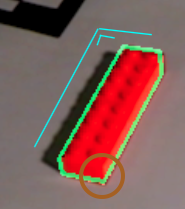
\includegraphics[width=0.5\linewidth]{img/brickPoseDetect}
  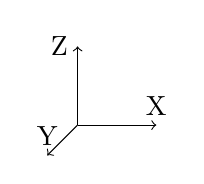
\begin{tikzpicture}
    \draw[->] (0,0,0) -- (0,0,1) node[above]{Y};
    \draw[->] (0,0,0) -- (0,1,0) node[left]{Z};
    \draw[->] (0,0,0) -- (1,0,0) node[above]{X};
  \end{tikzpicture}
  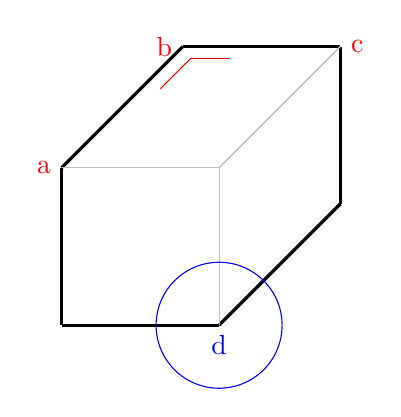
\begin{tikzpicture}
	\draw[black, very thick] (0,0 ,4) -- (2,0,4);
    \draw[black, very thick] (0 ,0,4) -- (0 ,2,4);
    \draw[black, very thick] (2,0 ,4) -- (2,0 ,0);
    \draw[black, very thick] (0 ,2,4) node[red,left]{a} -- (0 ,2,0);
    \draw[black, very thick] (2,0,0 ) -- (2,2,0 ) node[red,right]{c};
    \draw[black, very thick] (0,2,0 ) node[red,left]{b} -- (2,2,0 );
    
    \draw[lightgray] (0,2 ,4) -- (2,2 ,4);
    \draw[lightgray] (2 ,0,4) -- (2 ,2,4);
    \draw[lightgray] (2,2 ,4) -- (2,2 ,0);
    \draw[lightgray] (2 ,2,4) -- (2 ,2,0);
    \draw[lightgray] (2,0,4 ) -- (2,2,4 );
    \draw[lightgray] (0,2,4 ) -- (2,2,4 );
    
	\draw[red] (0.25,2 ,0.40) -- (0.75,2 ,0.40);
	\draw[red] (0.25,2 ,0.40) -- (0.25,2 ,1.40);
	
	\draw[blue] (2,0,4) node[blue,below]{d} circle (0.8);
  \end{tikzpicture}
  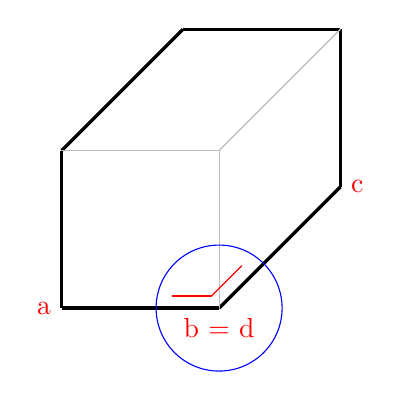
\begin{tikzpicture}
	\draw[black, very thick] (0,0 ,4) node[red,left]{a} -- (2,0,4);
    \draw[black, very thick] (0 ,0,4) -- (0 ,2,4);
    \draw[black, very thick] (2,0 ,4) -- (2,0 ,0);
    \draw[black, very thick] (0 ,2,4)  -- (0 ,2,0);
    \draw[black, very thick] (2,0,0 ) node[red,right]{c} -- (2,2,0 ) ;
    \draw[black,very thick] (0,2,0 ) -- (2,2,0 );
    
    \draw[lightgray] (0,2 ,4) -- (2,2 ,4);
    \draw[lightgray] (2 ,0,4) -- (2 ,2,4);
    \draw[lightgray] (2,2 ,4) -- (2,2 ,0);
    \draw[lightgray] (2 ,2,4) -- (2 ,2,0);
    \draw[lightgray] (2,0,4 ) -- (2,2,4 );
    \draw[lightgray] (0,2,4 ) -- (2,2,4 );
    
	\draw[red] (1.75,0 ,3.6) -- (1.25,0 ,3.6);
	\draw[red] (1.75,0 ,3.6) -- (1.75,0 ,2.6);
	
	\draw[blue] (2,0,4) node[red,below]{b = d}circle (0.8);
  \end{tikzpicture}
  \caption{Twee voorbeelden die aangeven hoe de pose vanuit een contour gevonden kan worden. }
  \label{fig:brickPoseDetect}
\end{figure}

Na het vinden van de contour moet hieruit worden achterhaald wat de pose van de legoblok is. Hiervoor bepalen we eerst in welk vlak van de legoblok elk hoekpunt van de contour ligt: onder- of bovenvlak. Dit geeft ons de $Z$ co\"ordinaat van al deze hoekpunten waardoor ze kunnen worden omgezet van 2D naar 3D via het pinhole model. Bij uitbreiding zijn dan alle hoekpunten van de legoblok in 3D gekend en dus kennen we ook de pose van de legoblok.

Eerst wordt uitgelegd hoe we kunnen achterhalen in welk vlak (boven of onder) elk hoekpunt van de contour ligt. Deze redenering wordt verduidelijkt met twee voorbeelden in figuur \ref{fig:brickPoseDetect}, waarin twee legoblokken worden getoond met hun contourlijnen aangeduid met de vette zwarte lijnen.

Uit de geometrische informatie van een legoblok weten we dat minstens drie opeenvolgende hoekpunten in hetzelfde Z-vlak liggen. Om te bepalen welke drie hoekpunten dit zijn zetten we alle 2D contourpunten om naar 3D (geprojecteerd op het grondvlak $Z = 0$) en bepalen we welke drie opeenvolgende 3D hoekpunten een hoek vormen die het dichtst bij 90 graden ligt (deze punten noemen we ($a$, $b$ en $c$). Van deze hoeken zijn we dan zeker dat ze in hetzelfde vlak liggen. In het eerste voorbeeld van figuur \ref{fig:brickPoseDetect} ligt de hoek tussen drie hoekpunten in het bovenvlak dichtst bij 0, in het tweede voorbeeld is dit de hoek op het grondvlak. Een ander geval is onmogelijk omdat, na projectie op het grondvlak, hoeken tussen punten in een verschillend $Z$-vlak sterker zullen afwijken van 90 graden.

Vervolgens bepalen we het hoekpunt ($d$) dat in 3D (opnieuw geprojecteerd op grondvlak $Z = 0$) zich het dichtst bij de camera bevindt, hiervan kan met zekerheid gezegd worden dat het werkelijk in het vlak $Z = 0$ ligt. Punten van het bovenvlak zijn namelijk na projectie verder van de camera verwijderd dan hun overeenkomstige punten op het grondvlak. Dit dichtstbijzijnde hoekpunt is in de voorbeelden aangeduid met een blauwe cirkel. Nu kan met zekerheid gezegd worden of $a$, $b$ en $c$ in het onder- of bovenvlak van de legoblok liggen: 
\begin{itemize}
\item Als $d == a$ $OF$ $d == b$ $OF$ $d == c$, dan liggen $a$, $b$ en $c$ in het ondervlak;
\item Anders liggen $a$, $b$ en $c$ in het bovenvlak.
\end{itemize}
In het eerste voorbeeld van figuur \ref{fig:brickPoseDetect} liggen de hoekpunten $a$, $b$ en $c$ dus in het bovenvlak aangezien hoekpunt $d$ niet gelijk is aan \'e\'en van deze hoeken. In het tweede voorbeeld is dit wel het geval en dus liggen de drie punten in het ondervlak. Dit geeft ons (via het pinhole model) de 3D posities van alle hoekpunten van de contour en bij uitbreiding van de volledige legoblok.

\subsection{Legoblok toevoegen aan de virtuele wereld} \label{sec:naive_algo_3}

Nu we de pose van de legoblok bepaald hebben wordt de legoblok toegevoegd aan de virtuele wereld. Om ervoor te zorgen dat blokken niet meermaals worden toegevoegd worden blokken die voldoende dicht bij elkaar liggen samengenomen met behulp van een voting mechanisme. Dit verloopt als volgt:

Wanneer elk hoekpunt van het ene legoblok dichter dan 0.8 cm ligt bij een hoekpunt van een reeds gedetecteerde blok worden deze blokken gezien als dezelfde blok. In dat geval kan gestemd worden op de grootte en positie van de blok door het gemiddelde te nemen van de groottes en posities van alle blokken die zo dicht bij elkaar liggen. De waarde 0.8 cm is niet toevallig gekozen: het is exact de helft van de breedte van een 2x2 legoblok, zo dicht kunnen legoblokken dus nooit bij elkaar liggen (dit is voor ons namelijk het kleinste legoblokje dat gedetecteerd kan worden).

Bovendien heeft een legoblok in de virtuele wereld nog een status waarin deze verkeert. De twee mogelijk statussen zijn om te bepalen wanneer de blok een deel van het spel wordt (\textit{actief}) en wanneer de blok er geen deel meer van uitmaakt (\textit{inactief}). Wanneer een blok minstens in drie frames werd gedetecteerd wordt hij actief, maar indien hij minstens drie frames achter elkaar niet werd gedetecteerd wordt hij inactief en wanneer hij na vijf frames achter elkaar niet is gedetecteerd wordt hij zelfs verwijderd. Dit mechanisme maakt het algoritme flexibeler om blokken te kunnen toevoegen of verwijderen uit het spel wanneer de speler dat wil.

\section{Implementatie, resultaten en evaluatie} \label{sec:naive_algo_result}

%\section{Evaluatiemethode en implementatie}
%In deze sectie bespreken we eerst kort op welke manier de performantie van beide algoritmes worden ge\"evalueerd. Vervolgens wordt kort overlopen welke machine en welke bibliotheken er zijn gebruikt voor de implementaties van de algoritmes.
%
%\subsection{Evaluatiemethode}
%
%\begin{figure}
%  \centering
%  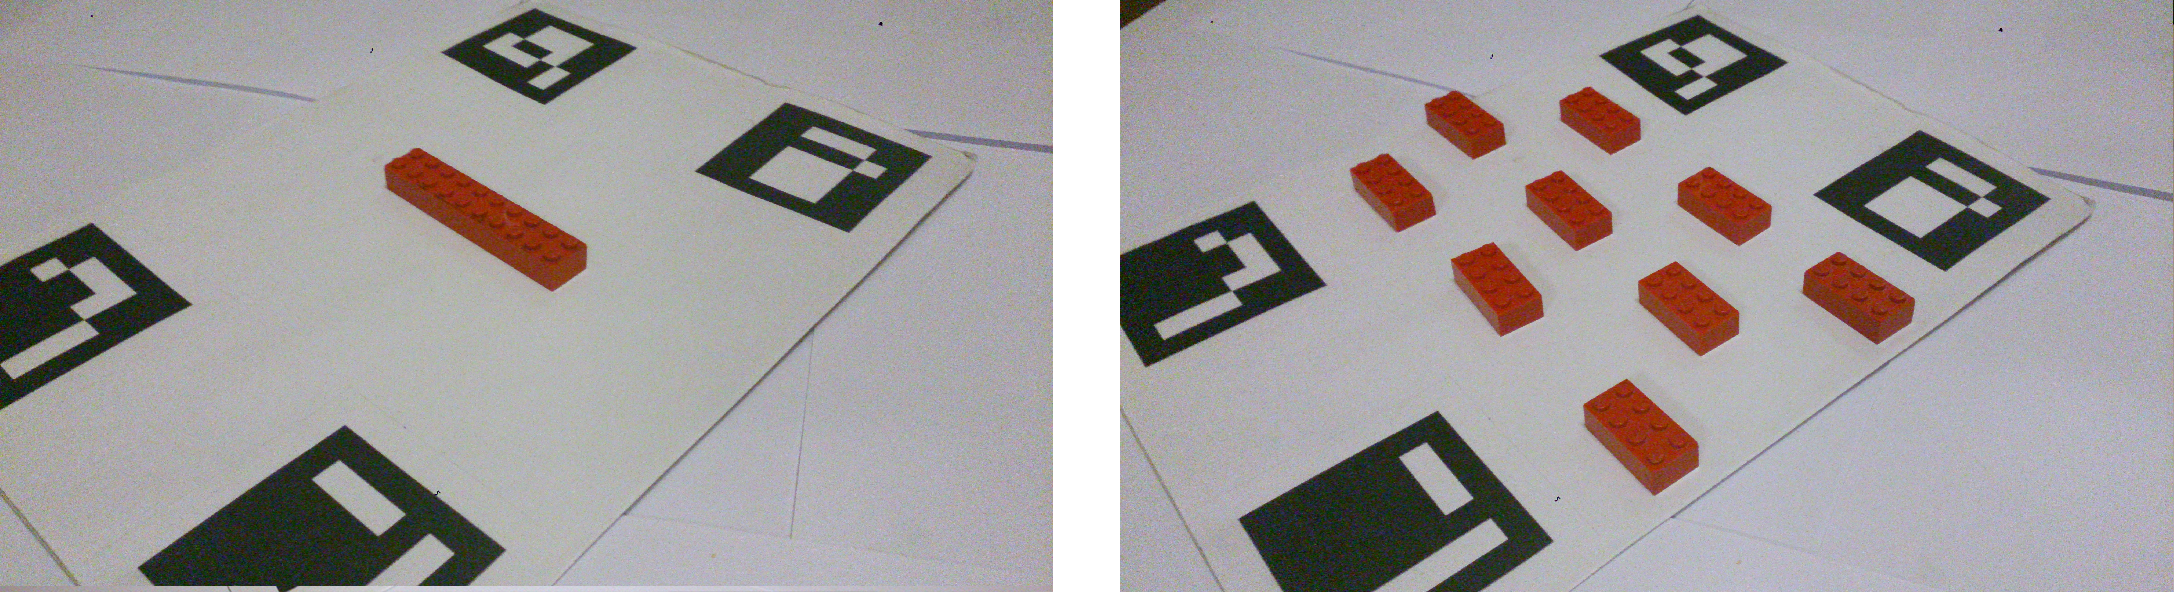
\includegraphics[width=\linewidth]{img/simpleComplex}
%  \caption{Simpele (links) en complexe scene (rechts) voor performantie evaluatie van na\"ieve blokdetectie.}
%  \label{fig:simple_complex}
%\end{figure}
%
%De performantie van beide algoritmes werden ge\"evalueerd door de tijd op te meten van het volledige lemmingenspel zowel wanneer een eenvoudige scene werd gebouwd als wanneer een complexe scene werd gebouwd. Figuur \ref{fig:simple_complex} toont beide scenes die hiervoor zijn gebruikt. Merk op dat dit scenes zijn die simpel en complex zijn voor deze algoritmes, maw. het zijn scenes die beide algoritmes kunnen detecteren en respectievelijk weinig / veel legoblokken bevatten.
%
%De opmeting gebeurde even lang als een lemming nodig heeft om van begin tot eindpunt te geraken. Aangezien de snelheid gedefinieerd is als 0.5 cm/s en de afstand minimum 23 cm is, duurt de opmeting dus minimum 11.5 seconden. Vervolgens wordt per opgemeten gedeelte het gemiddelde genomen om geen grote uitschieters te hebben.

\subsection{Implementatie}
De volledige implementatie en experimenten zijn uitgevoerd op een Sony Xperia Z C6602 met een Qualcomm Quad-core 1.5 GHz Krait processor, Adreno 320 GPU, 2GB RAM en Android 4.4.4 KitKat. Alles werd geprogrammeerd in Java 7 met gebruik van de Cardboard VR SDK van Google voor stereo rendering voor de Google Cardboard en de OpenCV 2.4.9 bibliotheek~\cite{opencv} voor implementaties van computer vision algoritmes.

De omzetting van YUV naar HSV werd ge\"implementeerd met de \texttt{cvtColor} methode van OpenCV. Voor de detectie van de contouren gebruikten we de \texttt{findContours} methode. Ten slotte werd ook nog de \texttt{approxPolyDP} methode gebruikt om de contouren met minder hoekpunten te beschrijven. Verder werden voornamelijk mathematische operaties van OpenCV gebruikt om de rest van het algoritme te implementeren.

\subsection{Resultaten}

\begin{figure}
  \centering
  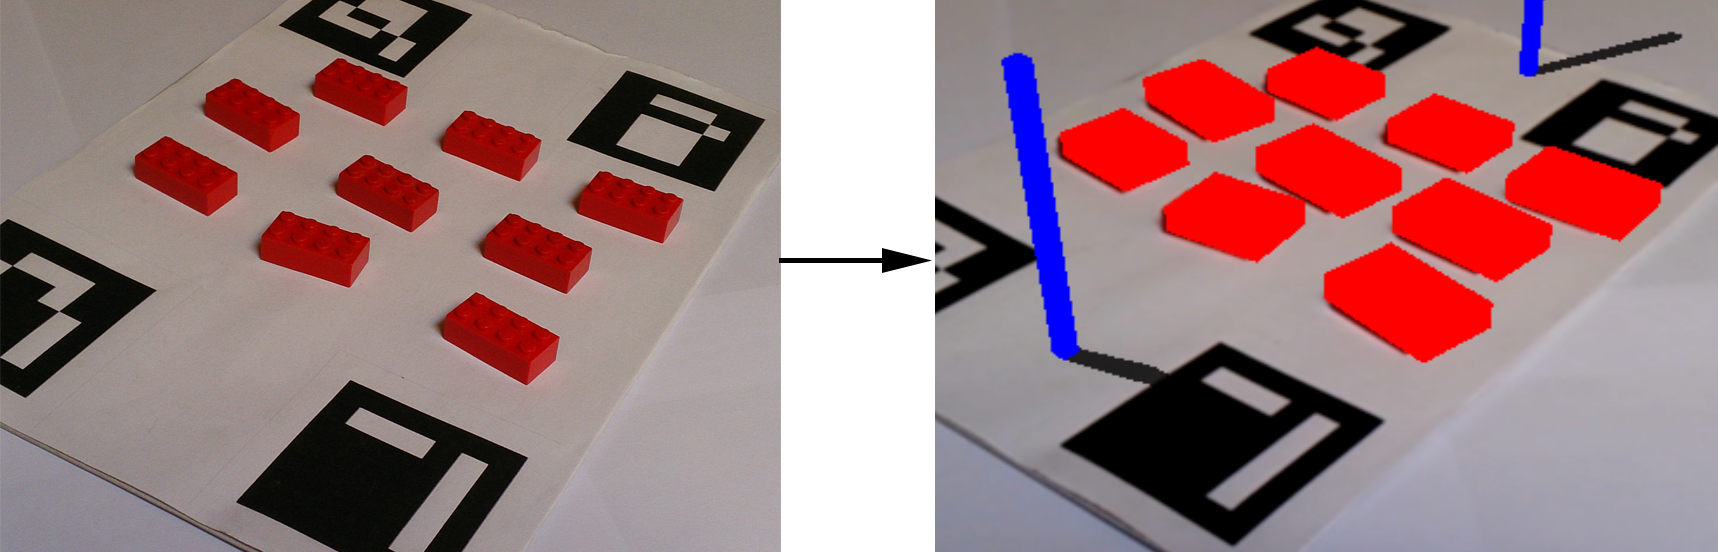
\includegraphics[width=\linewidth]{img/alg1}
  \caption{Resultaat van het na\"ieve algoritme.}
  \label{fig:result_algo1}
\end{figure}


Figuur \ref{fig:result_algo1} toont het resultaat van het algoritme. De linkerafbeelding toont de legoblokken en de rechterafbeelding wat de detectie van legoblokken oplevert. 

Merk op dat de rendering van de gedetecteerde legoblokken een kleine afwijking bevat van de werkelijke legoblokken. Dit wordt veroorzaakt door een trage performantie van het algoritme, waardoor de rendering in feite enkele frames oud is.

Verder valt ook op te merken dat de virtuele legoblokken iets groter zijn dan de werkelijke legoblokken. Dit is expliciet toegevoegd aan het algoritme omdat de virtuele wereld bestaat uit een discreet grid. Wanneer lemmings in dit discreet grid dan wandelen van node naar node kan het zijn dat ze deels in een legoblok wandelen omdat de blok niet exact stopt op een node. Om er dus zeker van te zijn dat de lemmings niet gedeeltelijk in een legoblok wandelen worden de virtuele legoblokken iets groter gemaakt dan de grootte van echte legoblokken.

\begin{figure}
  \centering
  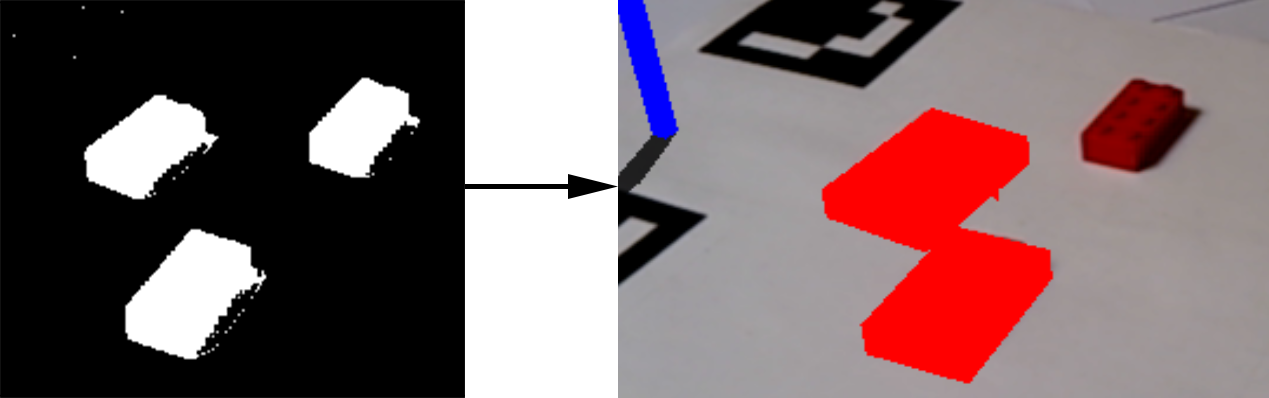
\includegraphics[width=\linewidth]{img/alg1Shadow}
  \caption{Resultaat van het na\"ieve algoritme bij veel schaduw.}
  \label{fig:algo1_shadow}
\end{figure}

In figuur \ref{fig:algo1_shadow} wordt aangetoond dat schaduw een negatief effect heeft op het resultaat van het algoritme. We zien in de threshold dat er wat artefacten op de plaats van de schaduw aanwezig zijn, dit resulteert uiteindelijk in legoblokken die moeilijk worden gevonden.

\begin{figure}
  \centering
  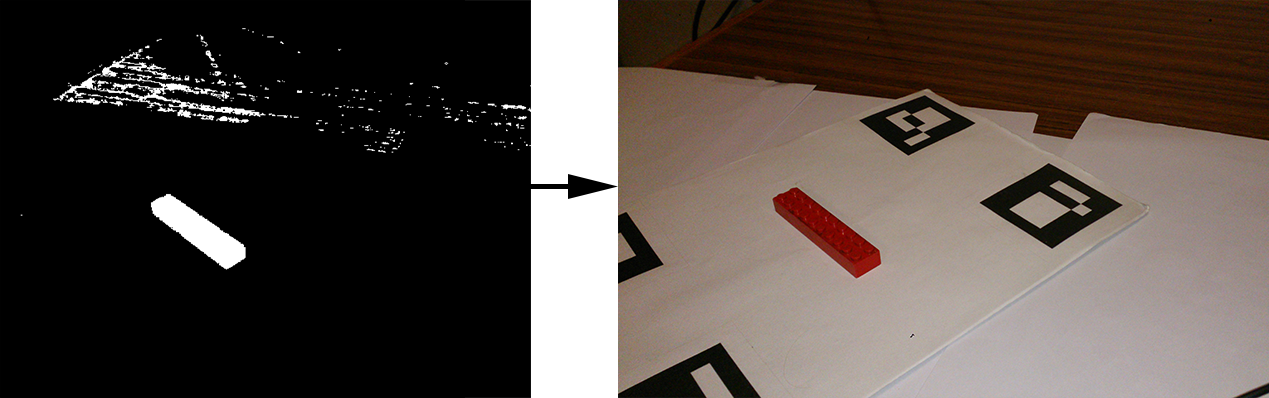
\includegraphics[width=\linewidth]{img/alg1NonWhiteBg}
  \caption{Resultaat van het na\"ieve algoritme bij rode tint in het beeld.}
  \label{fig:algo1_nonwhitebg}
\end{figure}

Omdat we kleurthresholding gebruiken is een rode tint in het beeld is absoluut uit den boze, elke kleur in het beeld dat een beetje in de grenzen van de threshold valt vormt een probleem. Dit tonen we aan in figuur \ref{fig:algo1_nonwhitebg}, waarin een bruine achtergrond in beeld komt. We zien duidelijk dat veel ruis in de threshold voorkomt. Het gevolg hiervan is vooral dat het algoritme een heel stuk trager is dan normaal: soms duren alle berekeningen samen wel tot 5 seconden. Dit komt omdat ruis in de threshold het algoritme doet denken dat op die plaatsen ook legoblokken staan en daardoor zal het al die contouren ook willen verwerken wat veel tijd vraagt. Bovendien gebeurde het zelden wel eens dat de camera zelf zijn belichting aanpaste (bijvoorbeeld wanneer plots grote hoeveelheden donkere kleuren in beeld komen), hierdoor werd de threshold voor de legoblok zelf ook slechter wat ertoe leidde dat de blok helemaal niet meer gedetecteerd werd.

\subsection{Performantie}

\subsubsection*{Evaluatiemethode}

\begin{figure}
  \centering
  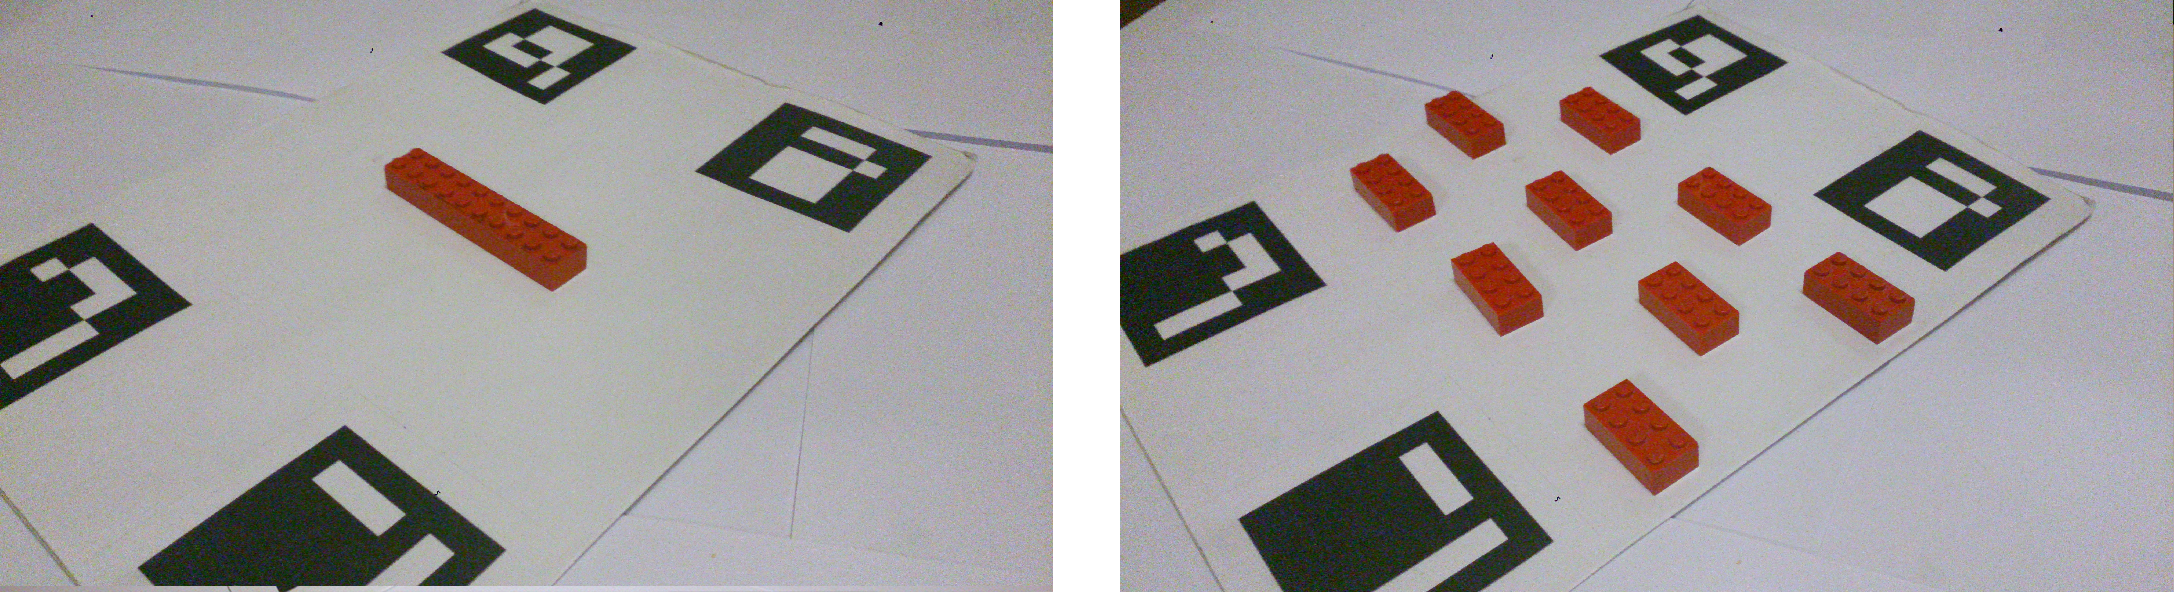
\includegraphics[width=\linewidth]{img/simpleComplex}
  \caption{Simpele (links) en complexe scene (rechts) voor performantie evaluatie van na\"ieve blokdetectie.}
  \label{fig:simple_complex}
\end{figure}

De performantie van werd ge\"evalueerd door de tijd op te meten van verschillende onderdelen van het algoritme terwijl een lemming loopt van het start- naar het eindpunt. Deze meting werd gedaan voor een eenvoudige en voor een complexe scene, zie figuur \ref{fig:simple_complex}. Merk op dat dit scenes zijn die simpel en complex zijn voor deze algoritmes, maw. het zijn scenes die beide algoritmes kunnen detecteren en respectievelijk weinig / veel legoblokken bevatten. Vervolgens werd per onderdeel het gemiddelde genomen van de gemeten tijd om geen grote uitschieters te hebben.

\subsubsection*{Evaluatie}

\begin{figure}
  \centering
  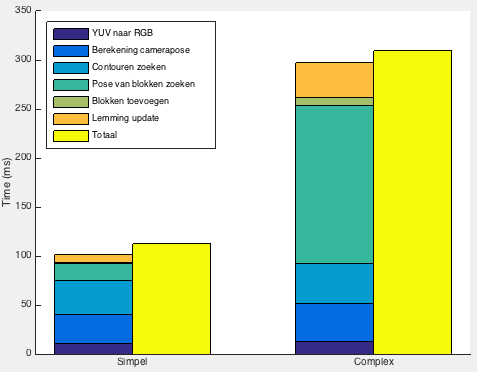
\includegraphics[width=.75\linewidth]{img/naivePerf}
  \caption{Gemiddelde performantie van het na\"ieve algoritme.}
  \label{fig:perf_algo1}
\end{figure}

Figuur \ref{fig:perf_algo1} toont de gemiddelde performantie van het na\"ieve algoritme voor de simpele scene (links) en complexe scene (rechts). De gele blok stelt telkens de totale tijd die het algoritme nodig heeft, de gekleurde blokken geven de onderverdelingen aan van deze tijd: 
\begin{itemize}
\item YUV omzetten naar RGB;
\item Camerapose berekenen (via markers);
\item Threshold berekenen en contouren van legoblokken zoeken (eerste deel van het algoritme);
\item Pose van de blokken zoeken (tweede deel van het algoritme);
\item Blokken toevoegen aan de virtuele wereld, mergen van blokken en voten voor grootte en positie van blokken (derde deel van het algoritme);
\item Lemmings updaten (oa. pad van de lemming updaten).
\end{itemize}
Merk op dat de som van de gekleurde blokken niet exact gelijk is aan de grootte van de gele blok. Dit komt omdat enkel de belangrijkste onderdelen uit het algoritme zijn opgenomen in deze grafiek, enkele implementatie specifieke details zijn weggelaten omdat ze erg weinig tijd innemen en onbelangrijk zijn.

In de grafiek zien we dat het zoeken van de pose erg veel verschilt tussen de complexe en simpele scene. Dit is normaal aangezien het aantal legoblokken hoger ligt en dus moet dit na\"ieve algoritme meer iteraties doen in een complexe scene. Het zoeken van contours daarentegen duurt niet significant langer in een complexe sc\`ene. De verklaring hiervoor is dat het bepalen van de kleurthreshold, wat in beide gevallen slechts eenmaal moet gebeuren, het langst duurt en dat de rest van de berekeningen, die even vaak moeten gebeuren als het aantal gedetecteerde legoblokken, slechts een zeer kleine bijdrage zijn. 

We merken ook op dat het updaten van de lemmingen een stuk langer duurt, dit is ook aannemelijk omdat bij de complexe scene het pad van een lemming van begin tot eindpunt een stukje langer is dan bij de simpele scene. De lemming moet immers om elke muur heen lopen en niet slechts om \'e\'en legoblokje. Aangezien dit pad ook steeds opnieuw wordt berekend (om \textit{on-the-fly} toevoegen van blokken toe te kunnen staan) is dit verschil significant.

Als we kijken naar de totale tijd de volledige berekening inneemt, dan wordt duidelijk dat dit algoritme erg traag is. Het komt neer op 8.9 fps voor de simpele scene en 3.2 fps voor de complexe scene, wat natuurlijk erg traag is voor een AR spel.

\begin{figure}
  \centering
  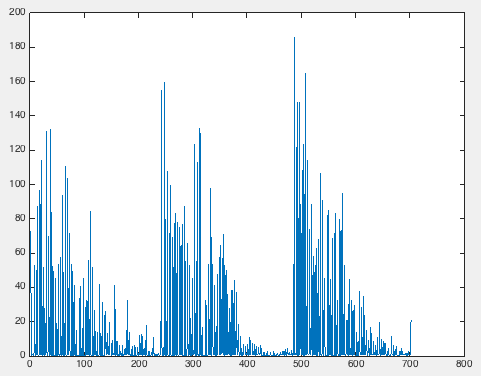
\includegraphics[width=.75\linewidth]{img/naiveLemmPerf}
  \caption{Gemiddelde performantie van het "Lemming updaten" onderdeel van het na\"ieve algoritme.}
  \label{fig:naive_lemm_perf}
\end{figure}

Figuur \ref{fig:naive_lemm_perf} geeft weer hoe de performantie van het updaten van de lemming veranderd gedurende het spel. Hiervoor hebben we de lemming drie maal laten lopen van start- tot eindpunt. We zien duidelijk een performantie van orde $O(1/x)$ die zichzelf telkens herhaalt. Wanneer de lemming namelijk dichter bij het eindpunt komt wordt het pad tot het eindpunt steeds korter en dus duurt het zoeken van het pad steeds minder lang tot het moment dat hij het eindpunt heeft bereikt. Hierna zal een nieuwe lemming starten vanaf het beginpunt waardoor het terug lang duurt om het pad te zoeken. We zien hier drie iteraties omdat drie lemmingen hebben gewandeld van begin- tot eindpunt.

Merk ook op dat de tijdsduur regelmatig voor een korte tijd bijna nul is. Dit komt omdat we de lemming updaten aan een constante snelheid, dus ongeacht hoe lang het volledige algoritme erover doet de lemming zal steeds aan constante snelheid lopen. Dit kan ervoor zorgen dat de lemming tijdens de volgende lemming update de volgende node nog niet heeft bereikt waardoor voorlopig nog geen nieuw pad wordt berekent. Omdat dan geen pad wordt berekent valt de zwaarste berekening van het onderdeel "Lemming updaten" weg en dus is de tijdsduur van dit onderdeel dan zo goed als nul.

\subsection{Besluit} \label{sec:naive_sub_besl}
Deze na\"ieve implementatie heeft \'e\'en belangrijk voordeel:
\begin{itemize}
\item Ze laat toe dat legoblokken \textit{on-the-fly} worden toegevoegd aan de virtuele wereld.
\end{itemize}

Aan deze methode zijn echter meer nadelen verbonden:
\begin{itemize}
\item Legoblokken mogen niet in een hoek naast elkaar staan omdat dan de veronderstelling dat een contour maximaal zes hoeken bevat niet meer geldig is.
\item Enkel rode legoblokken kunnen worden gedetecteerd. Dit nadeel is echter eenvoudig weg te werken zoals wordt besproken in sectie \ref{sec:naive_vereenv}.
\item Legoblokken mogen niet in meerdere niveau's gebouwd worden. Muren (meerdere legoblokken op elkaar maar de breedte en de lengte van de constructie is op elk niveau gelijk) zouden in principe wel kunnen (ze hebben immers maximaal zes hoekpunten) maar dan moet op \'e\'en of andere manier de grootte van deze muur bepaald worden, dit wordt uitgebreider behandeld in hoofdstuk \ref{hoofdstuk:4}. Andere constructies in de hoogte kunnen echter niet omdat we dan meer dan zes hoekpunten deel kunnen uitmaken van de contour.
\item Het algoritme kan niet goed om met veranderingen qua belichting. Dit komt omdat we puur thresholden op basis van kleur maar deze waarden zijn sterk afhankelijk van welke belichting we gebruiken. In hoofdstuk \ref{hoofdstuk:4} komt een calibratiemethode aan bod die dit probleem verhelpt.
\item Zoals aangegeven in de resultaten geeft een rode tint in het beeld een erg slecht resultaat, vooral qua performantie.
\item Performantie is erg laag.
\end{itemize}

Om een deel van deze nadelen weg te werken en bovendien de berekening van de pose eenvoudiger te maken voeren we in de volgende sectie een vereenvoudiging van dit algoritme in.
 
\section{Vereenvoudiging: blokdetectie met behulp van een 2D grid} \label{sec:naive_vereenv}
In deze vereenvoudiging zullen we in plaats van werkelijk de pose en positie van de legoblok te bepalen enkel de threshold gebruiken. Deze wordt dan over het grid van de virtuele wereld gelegd om te bepalen welke nodes niet toegankelijk zijn. Eerst behandelen we de aanpassingen ten opzichte van het vorige algoritme, vervolgens bespreken we de gevolgen die deze aanpassingen hebben en ten slotte de resultaten en performantie van deze vereenvoudigde versie.

\subsection{Algoritme}
Het eerste deel van het na\"ieve algoritme wordt sterk ingekort aangezien we enkel een threshold nodig hebben. Maar er zijn ook een tweetal toevoegingen om tegemoet te komen aan de nadelen van het algoritme:

Ten eerste berekenen we opnieuw een kleurthreshold maar deze keer niet enkel voor de kleur rood, ook voor geel en blauw. Op die manier  willen we aantonen dat het algoritme zonder problemen met meerdere kleuren overweg kan. Dit zijn kleurengrenzen die werden gebruikt om in een HSV afbeelding te thresholden zodat het resultaat een afbeelding is waarin de legoblokken wit zijn en de achtergrond zwart:
\begin{align*}
Rood: 160 < H < 180; 153 < S < 255; 30 < V < 255 \\
Geel: 135 < H < 160; 147 < S < 255; 30 < V < 255 \\
Blauw: 0 < H < 112; 42 < S < 255; 13 < V < 255
\end{align*}

\begin{figure}
  \centering
  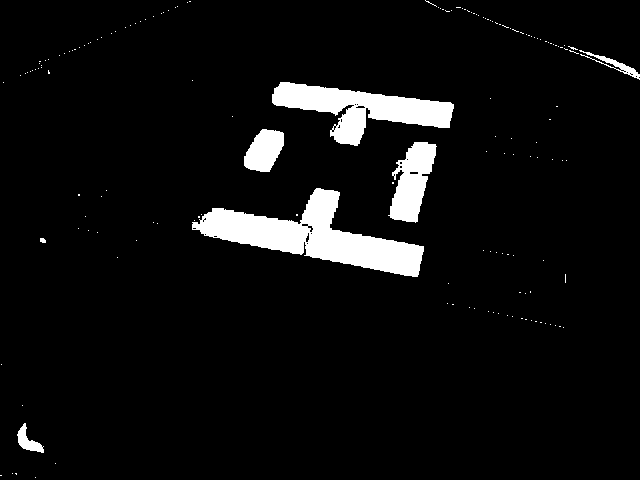
\includegraphics[width=0.5\linewidth]{img/alg2Noise}
  \caption{Ruis in threshold v\'o\'or morfologische operaties werden toegepast.}
  \label{fig:algo2_noise}
\end{figure}

Ten tweede, omdat we nu thresholden op meerdere kleuren kan het gebeuren dat er wat ruis optreedt in onze threshold. Deze ruis vertoont zich in hoopjes witte of zwarte lijntjes op plaatsen waar het niet hoort (zie figuur \ref{fig:algo2_noise}). Om dit te vermijden worden de morfologische operaties \textit{open} en \textit{close} toegepast op de threshold.

Het tweede en derde deel van het vorige algoritme (zie secties \ref{sec:naive_algo_2} en \ref{sec:naive_algo_3}) valt volledig weg, logisch want we hebben geen contour bepaald. In plaats daarvan worden alle nodes van het grid van onze virtuele wereld naar 2D omgezet (via het pinhole model). Dit 2 dimensionaal grid kunnen we vervolgens overlappen met de eerder berekende threshold en wanneer een node van de virtuele wereld zich in een witte regio van de threshold bevindt beschouwen we deze als ontoegankelijk. Omdat we enkel de nodes die tijdens het A* algoritme worden ge\"exploreerd moeten omzetten naar 2D, doen we dit tijdens de berekening van het pad en enkel voor de nodes die worden ge\"exploreerd.

\subsection{Gevolgen}
Deze vereenvoudiging is een grove versimpeling van het eerste algoritme aangezien de positie en grootte van een legoblok niet meer expliciet worden bepaald. Nu vragen we ons af welke consequenties dat heeft.

\begin{figure}
  \centering
  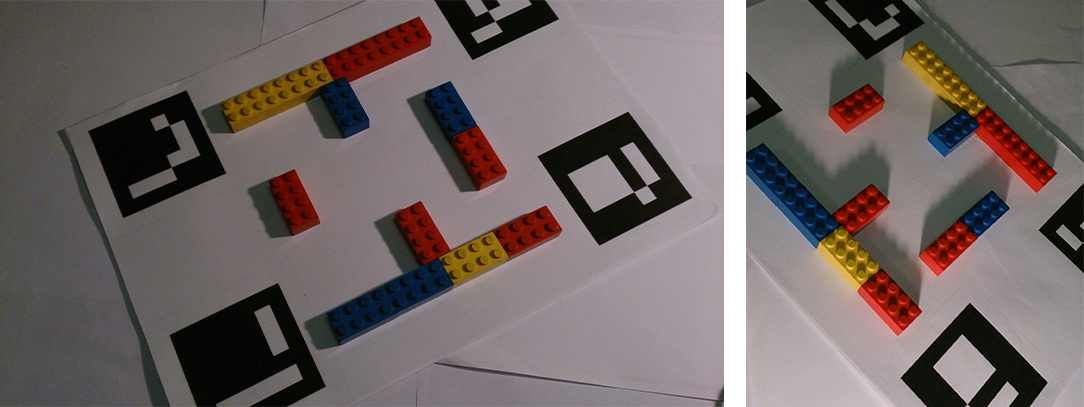
\includegraphics[width=\linewidth]{img/alg2Shadow}
  \caption{Fout van het vereenvoudigde na\"ieve algoritme in de vorm van schaduw.}
  \label{fig:algo2_shadow}
\end{figure}

Ten eerste wordt een fout gemaakt in het aantal nodes die bezet zijn door een legoblokje. Deze fout wordt gemaakt omdat een onbezet deel schuilt achter de legoblok waardoor dit niet zichtbaar is in de threshold en deze delen dus onterecht als ontoegankelijk worden beschouwd. Sterker nog: we kunnen precies defini\"eren dat die fout even groot is als de schaduw op het grondvlak wanneer een lichtbron vanuit de camera schijnt in dezelfde richting als de camera kijkt. Afbeelding \ref{fig:algo2_shadow} toont de fout in de vorm van schaduw als de camera op de plaats van de lichtbron zou staan. We zien dat de fout relatief klein is wanneer de camera hoog boven het grondvlak zou staan (links) en groter wordt wanneer de camera dichter naar het grondvlak toe zou bewegen (rechts).

Ten tweede heeft deze vereenvoudiging ook een aantal voordelen in die zin dat het enkele nadelen uit het na\"ieve algoritme wegwerkt:
\begin{itemize}
\item Legoblokken in meerdere kleuren kunnen gebruikt worden, het gevolg is wel dat morfologische operaties de threshold moeten oppoetsen om er ruis uit te halen zie figuur \ref{fig:algo2_noise}. Dit werd hoogstwaarschijnlijk veroorzaakt door de belichting die niet altijd constant is, zodat de thresholdwaarden niet altijd even nauwkeurig zijn. Merk op dat dit even goed in het eerste algoritme had kunnen worden ge\"implementeerd.
\item Legoblokken kunnen nu ook in een hoek tegen elkaar staan, wat bij het na\"ieve algoritme niet was toegestaan. Een nadeel is echter wel dat meerdere niveau's in dit algoritme helemaal uitgesloten zijn, terwijl dit in theorie in het vorige algoritme wel was toegestaan (met bepaalde restricties). Dit komt omdat wanneer we de constructie hoger maken, de fout van deze vereenvoudiging steeds groter wordt. Er is immers een nog groter gedeelte van het grondvlak, waar geen legoblokken op staan, verborgen achter de legoblokconstructie.
\end{itemize}

\subsection{Implementatie} \label{naive_vereenv_impl}
De morfologische operaties werden ge\"implementeerd met behulp van de \texttt{morphologyEx} functie van OpenCV. Deze operatie werd in dit algoritme gebruikt om eerst een \textit{close} operatie met een ellipsvormige kernel van 9x9 en vervolgens een \textit{open} operatie met een ellipsvormige kernel van 17x17 uit te voeren op de kleurthreshold. Experimenteel werd ondervonden dat deze parameters het beste werken.

Verder werd er ook voor gekozen om niet elke keer het volledige grid van de virtuele wereld om te zetten van 3D naar 2D. In plaats hiervan worden enkel de nodes van het grid omgezet die ge\"exploreerd worden door het A* algoritme. Deze keuze is een kwestie van performantie: ten eerste omdat het grid elke keer opnieuw van 3D naar 2D moet worden omgezet (de pose van de camera is immers elke keer verschillend) en ten tweede omdat in het A* algoritme bijna nooit alle nodes worden ge\"exploreerd.

\subsection{Resultaten en performantie} \label{naive_vereenv_res}

\subsubsection*{Resultaten}
Voor deze vereenvoudiging is het niet mogelijk om een rendering te maken van de virtuele legoblok (zoals bij het eerste algoritme in sectie \ref{fig:result_algo1}). Dit komt omdat de legoblokken in principe nooit volledig worden berekend: er wordt enkel een threshold gebruikt waar vervolgens een grid over wordt gelegd.

\begin{figure}
  \centering
  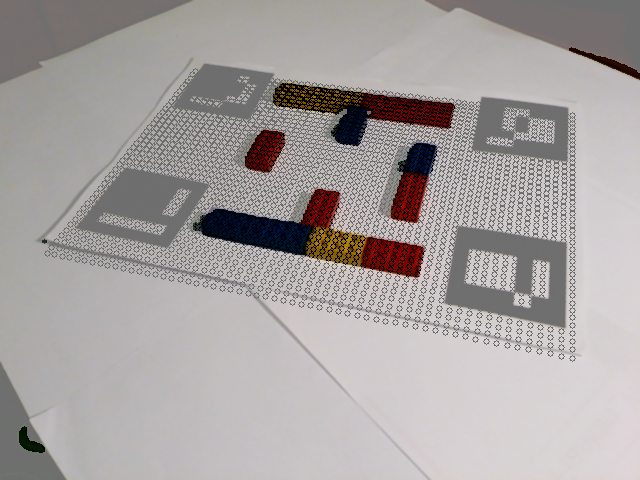
\includegraphics[width=.5\linewidth]{img/alg2}
  \caption{Resultaat van het tweede na\"ieve algoritme.}
  \label{fig:algo2_res}
\end{figure}

Figuur \ref{fig:algo2_res} toont het resultaat door het zwarte deel van de threshold deels transparant te maken. We kunnen duidelijk zien dat de legoblokken goed werden gedetecteerd via kleurthresholding. Ook werd over het grondvlak het grid gelegd, hierdoor is het duidelijk welke nodes niet toegankelijk zijn voor lemmings.

\subsubsection*{Performantie}

\begin{figure}
  \centering
  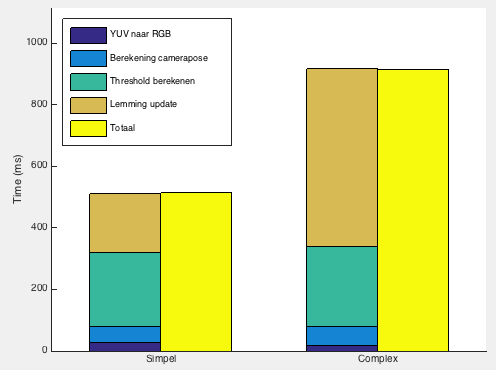
\includegraphics[width=.75\linewidth]{img/naiveVereenvPerf}
  \caption{Gemiddelde performantie van de vereenvoudiging van het na\"ieve algoritme.}
  \label{fig:naive_vereenv_perf}
\end{figure}

Figuur \ref{fig:naive_vereenv_perf} toont de gemiddelde performantie van de vereenvoudiging van het na\"ieve algoritme voor de simpele scene (links) en complexe scene (rechts). Opnieuw stelt de gele blok de totale tijd voor en de gekleurde blokken zijn de onderverdelingen van de totale tijd. Omdat in deze vereenvoudiging een deel van het oorspronkelijke algoritme niet meer wordt gebruikt is de onderverdeling ook licht anders:
\begin{itemize}
\item YUV omzetten naar RGB;
\item Camerapose berekenen (via markers);
\item Threshold berekenen;
\item Lemmings updaten (oa. pad van de lemming updaten en grid vergelijken met threshold).
\end{itemize}

Het belangrijkste dat we kunnen opmaken uit deze figuur is dat de totale tijd van deze vereenvoudiging meer dan dubbel zoveel is als de totale tijd van het oorspronkelijke algoritme. Deze vereenvoudiging kunnen we dus niet echt een verbetering noemen op vlak van performantie. Dit komt enerzijds omdat we elke keer opnieuw een volledig pad moeten berekenen en dus ook veel nodes moeten omzetten van 3D naar 2D. Anderzijds komt dit ook omdat de berekening van de threshold veel langer duurt dan de berekening van de contour bij het oorspronkelijke algoritme. De oorzaak hiervan vinden we bij het gebruik van meerdere kleuren waardoor ook enkele morfologische operaties nodig zijn wat erg dure operaties zijn.

We zien ook dat de berekening van de threshold in beide gevallen ongeveer even lang duurt: dit komt omdat een threshold berekenen onafhankelijk is van het aantal legoblokken dat wordt gedetecteerd. Het updaten van de lemmings duurt echter significant langer bij de complexe sc\`ene. Dit is normaal omdat het pad van de lemming dan langer is waardoor er dus meerdere nodes worden ge\"exploreerd en dus ook meer die van 3D naar 2D moeten worden omgezet.

\subsection{Besluit}
Deze vereenvoudiging maakte het algoritme veel simpeler en loste ook enkele nadelen op. Helaas is dit algoritme wel erg traag en laat het ons helemaal niet toe om legoconstructies met meerdere niveau's te gebruiken.

Om het performantieprobleem te verhelpen breiden we in de volgende sectie dit algoritme nog eenmaal uit. In deze uitbreiding vervangen we het A* algoritme met Tree Adaptive A* om paden te zoeken in de virtuele wereld. In deze uitbreiding zullen grote delen van reeds berekende paden herbruikbaar zijn waardoor per frame minder nodes van 3D naar 2D moeten worden omgezet.
 
\section{Uitbreiding: Tree Adaptive A*} \label{sec:naive_uitbr}
In deze sectie leggen we uit hoe Tree Adaptive A* (Tree-AA*) werkt en in welke mate het de performantie heeft verhoogd. Dit algoritme is in dieper detail uitgelegd in~\cite{hernandez2011tree}.

\subsection{Algoritme}

\begin{figure}
  \centering
  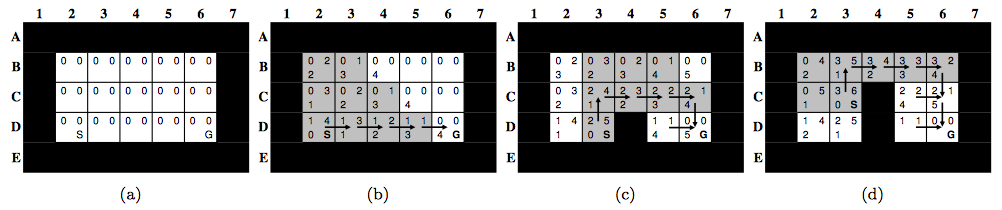
\includegraphics[width=\linewidth]{img/TAAStar}
  \caption{Voorbeeld van het Tree Adaptive A* algoritme (uit~\cite{hernandez2011tree}).}
  \label{fig:taastar}
\end{figure}

Tree Adaptive A* is een algoritme dat een uitbreiding is op Path Adaptive A*, wat op zijn beurt een uitbreiding is op Adaptive A*. Het algoritme gaat uit van de \textit{freespace} assumptie, waarin een agent zich een pad door een onbekend terrein moet banen naar een doelcel. Met een onbekend terrein bedoelen we dat hij niet weet waar obstakels zijn, hij kan deze enkel om zich heen voelen. Hierdoor zal de agent elke keer hij een onbekend obstakel voelt het pad met optimale kost moeten aanpassen. Bij elke aanpassing mag de agent wel gebruik maken van de suffixen van vroeger berekende minimale kost paden (behalve natuurlijk de stukjes paden die door het obstakel gingen). De vorige paden die herbruikbaar zijn worden steeds opgeslagen in een datastructuur die de \textit{herbruikbare boom} wordt genoemd (het is namelijk een boom met zijn wortel in de doelcel). Zo moet de agent telkens slechts een deel van het pad aanpassen wat het zoeken van een pad een heel stuk effici\"enter maakt. De grootste kost zit dan in de initi\"ele zoektocht van een pad maar aangezien de meeste obstakels dan nog niet door de agent kunnen worden gezien zal dit best meevallen. 

We zetten onze uitleg nog kracht bij met het voorbeeld dat ook werd aangehaald in de paper (\cite{hernandez2011tree}), zie figuur \ref{fig:taastar}. Alle grijze tegels zijn ge\"expandeerde nodes en de zwarte tegels zijn de obstakels waar de agent weet van heeft. Figuur \ref{fig:taastar}a toont het beginsituatie, figuur \ref{fig:taastar}b toont de situatie waarin gezocht wordt naar een pad met minimale kost tot de doelcel. Nog geen obstakels zijn gevonden omdat deze zich niet bevinden rondom de huidige cel van de agent (cel D1). Het zoeken stopt wanneer de agent net cel D6 wil gaan expanderen, het resulterende pad is dan [D1, D2, D3, D4, D5, D6]. De agent gaat dan naar cel D3 en voelt van daaruit een obstakel in cel D4. Het vorige minimale kost pad deels verwijderd omdat dit door het obstakel ging. Het stukje tussen D5 en D6 blijft echter over in de \textit{herbruikbare boom} omdat dit nog steeds deel kan uitmaken van een minimaal kost pad (we weten immers niet of op plaats D5 ook een obstakel zou liggen). De agent vindt vervolgens een nieuw pad dat ook aan de boom wordt toegevoegd. In de laatste stap wordt een obstakel ontdekt in cel C4 waardoor het stuk pad [D3, C3, C4, C5] verdwijnt uit de boom terwijl het stukje [C5, C6, D6] in de boom blijft. Bij het vinden van het nieuwe pad wordt het stukje [C6, D6] herbruikt.

Het grote voordeel aan dit algoritme voor een AR spel is dat deze \textit{herbruikbare boom} kan gedeeld worden tussen lemmingen. Dus als de wereld niet veranderd moeten weinig stukjes pad herberekend worden.

\subsection{Performantie}

\begin{figure}
  \centering
  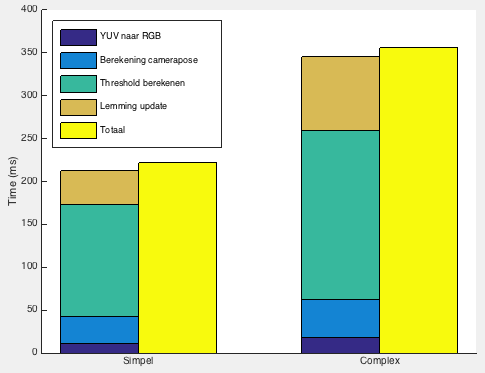
\includegraphics[width=.75\linewidth]{img/naiveTAAPerf}
  \caption{Gemiddelde performantie van de uitbreiding op de vereenvoudiging van het na\"ieve algoritme.}
  \label{fig:naive_uitbr_perf}
\end{figure}

Figuur \ref{fig:naive_uitbr_perf} toont de gemiddelde performantie van de uitbreiding op de vereenvoudiging van het na\"ieve algoritme voor de simpele scene (links) en complexe scene (rechts). Opnieuw stelt de gele blok de totale tijd voor en de gekleurde blokken zijn de onderverdelingen van de totale tijd.

We zien dat de totale tijd is afgenomen ten opzichte van de niet-uitgebreide versie van het algoritme. De performantie is echter wel nog steeds lager dan bij de oorspronkelijke versie. Dit wordt veroorzaakt door de tijd die de morfologische operaties nodig hebben (zoals eerder aangegeven in sectie \ref{sec:naive_vereenv_res}). Het is wel zo dat de tijd om een pad te zoeken van de lemming zoals verwacht sterk is afgenomen. Het is zelfs zo sterk afgenomen dat het berekenen van de threshold veel langer duurt dan alle andere operaties.

Het is bovendien opmerkelijk dat er geen significante verhoging is van de performantie tussen de simpele en complexe sc\`ene. Erg onlogisch is dit natuurlijk niet voor de berekening van de camera pose, omzetten van YUV naar RGB of berekenen van de threshold aangezien dit onafhankelijk is van het aantal gedetecteerde legoblokken. Bij het updaten van de lemming is dit echter wel opmerkelijker aangezien het pad langer is maar door het gebruik van Tree Adaptive A* duurt het gemiddeld gezien telkens even lang. Dit toont aan dat dit algoritme robuust is tegen een verhoging van het aantal legoblokken in de sc\`ene.

\section{Besluit} \label{sec:naive_besl}
In dit hoofdstuk werd een na\"ief algoritme voorgesteld dat op basis van een kleurthreshold en geometrische eigenschappen legoblokken detecteert. Dit algoritme had echter een heleboel nadelen: oa. konden legoblokken niet in een hoek tegen elkaar staan, konden enkel rode legoblokken worden gedetecteerd en was de performantie erg laag. Daarom werd een vereenvoudiging van dit algoritme voorgesteld waarin de pose van een legoblok niet expliciet werd berekent. In plaats daarvan werd het 3D grid van de virtuele wereld over de threshold gelegd om te bepalen welke nodes ontoegankelijk waren. Het probleem was echter dat de performantie nog lager was dan het oorspronkelijke algoritme. Daarom werd het Tree Adaptive A* algoritme ingevoerd maar hoewel de performantie wel een heel stuk beter was, was het nog steeds niet te vergelijken met de performantie van het oorspronkelijke algoritme (voornamelijk door de morfologische operaties). Een ander nadeel van het vereenvoudigde algoritme was dat nu helemaal niet meer in de hoogte kon worden gebouwd omdat dit de fout van dit algoritme enkel groter maakt.

In het volgende hoofdstuk gaan we op zoek naar een methode waarmee ook legoconstructies met meerdere niveau's gedetecteerd kunnen worden. Om dit te verwezenlijken proberen we alle geometrische informatie te gebruiken die een legoblok bevat (niet slechts enkele eigenschappen zoals dit algoritme deed). 

%%% Local Variables: 
%%% mode: latex
%%% TeX-master: "masterproef"
%%% End: 
